%
% s-perihel.tex -- relativistische Periheldrehung, numerisch berechnet
%
% (c) 2017 Prof Dr Andreas Müller, Hochschule Rappersiwl
%

\section{Periheldrehung%
\label{skript:chapters:s-perihel}}
\rhead{Periheldrehung}
\begin{figure}
\centering
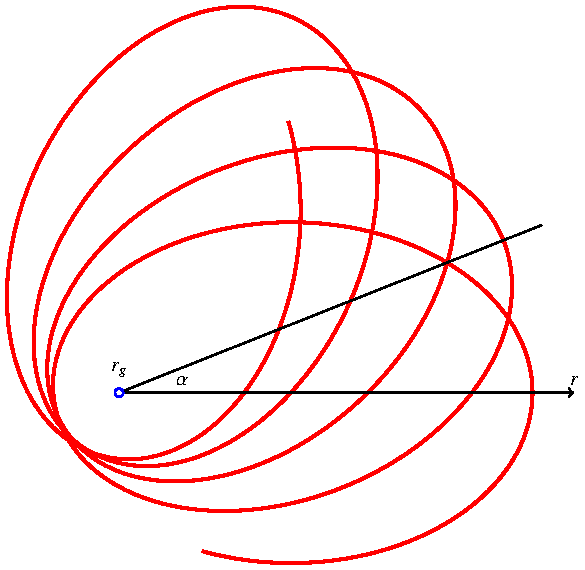
\includegraphics{chapters/tikz/orbit.pdf}
\caption{Periheldrehung um den Winkel $\alpha$ in jedem Umlauf um den
Zentralkörper in einer Schwarzschild-Metrik mit Anfangsbedingungen
\label{skript:schwarzschild:anfangsbedingung:normal}.
\label{skript:schwarzschild:perihelorbit}}
\end{figure}
Das erste Keplersche Gesetz sagt, dass ein Planet sich auf einer
Ellipsenbahn bewegt.
Die Newtonsche Gravitationstheorie bestätigt dies, die Differentialgleichungen
für das Zweikörperproblem sind in geschlossener Form lösbar.
Insbesondere zeigt die Richtung zum sonnennächsten Punkt, dem Perihel,
immer in die gleiche Richtung.
Für die Merkurbahn wurde jedoch eine Abweichung festgestellt, die
Perihelrichtung dreht sich mit der Zeit um die Sonne.
Einen Teil dieser Drehung konnte mit der newtonschen Theorie erklärt werden.
So führen zum Beispiel die Abplattung der Sonne und die Störungen durch
andere Planeten zu einem solchen Effekt.
Von den gemessenen $571.91''$ Periheldrehung des Merkur pro Jahrhundert
verblieben jedoch $43.11''$ pro Jahrhundert, die die Newtonsche
Theorie nicht erklären konnte.


Schon in seinem ursprünglichen Entwurf der allgemeinen Relativitätstheorie
hat Einstein die durch die Abweichung von der Newtonschen Theorie
verursachte Periheldrehung der Merkurbahn berechnet und gute Übereinstimmung
mit der bekannten Drehung gefunden.
Damit hat er bereits selbst eine erste experimentelle Bestätigung
der Theorie gegeben.

Um den Effekt überhaupt darstellen zu können, muss die Bahn sehr nahe
am Zentralkörper vorbeiführen, der nächste Punkt, das Apastron darf
also nur wenige Gravitationsradien entfernt sein.
In Abbildung~\ref{skript:schwarzschild:perihelorbit} ist die
Umlaufbahn eines Körpers dargestellt, dessen Apastron-Entfernung
$100 r_g$ ist und der sich im Periastron auf etwa $20r_g$ 
nähert.
Die Apsidenlinie dreht sich hier in jedem Umlauf um $\alpha = 21.61^\circ$.
Ziel dieses Abschnittes ist zu zeigen, wie die Periastron-Drehung
in einer Schwarzschild-Metrik numerisch berechnet werden kann.
Es geht dabei nicht darum, den exakten Wert für die Periheldrehung
des Merkur zu bestimmen,
sondern nur zu zeigen, dass die allgemeine Relativitätstheorie
qualititativ einen solchen Effekt vorhersagt.

\subsection{Geodätengleichung für die Schwarzschild-Metrik}
\label{skript:schwarzschild:geodaetengleichung}
%(%i5) 		        ratsimp(Christoffel2(1, 1, 1))
%(%o5) 				       0
%(%i6) 		        ratsimp(Christoffel2(1, 1, 2))
%				       rg
%(%o6) 			        - -------------
%					      2
%				  2 r rg - 2 r
%(%i7) 		        ratsimp(Christoffel2(1, 1, 3))
%(%o7) 				       0
%(%i8) 		        ratsimp(Christoffel2(1, 1, 4))
%(%o8) 				       0
%(%i9) 		        ratsimp(Christoffel2(1, 2, 2))
%(%o9) 				       0
%(%i10) 		        ratsimp(Christoffel2(1, 2, 3))
%(%o10) 				       0
%(%i11) 		        ratsimp(Christoffel2(1, 2, 4))
%(%o11) 				       0
%(%i12) 		        ratsimp(Christoffel2(1, 3, 3))
%(%o12) 				       0
%(%i13) 		        ratsimp(Christoffel2(1, 3, 4))
%(%o13) 				       0
%(%i14) 		        ratsimp(Christoffel2(1, 4, 4))
%(%o14) 				       0
%(%i15) 		        ratsimp(Christoffel2(2, 1, 1))
%				     2
%				   rg  - r rg
%(%o15) 				 - ----------
%					 3
%				      2 r
%(%i16) 		        ratsimp(Christoffel2(2, 1, 2))
%(%o16) 				       0
%(%i17) 		        ratsimp(Christoffel2(2, 1, 3))
%(%o17) 				       0
%(%i18) 		        ratsimp(Christoffel2(2, 1, 4))
%(%o18) 				       0
%(%i19) 		        ratsimp(Christoffel2(2, 2, 2))
%				      rg
%(%o19) 				 -------------
%					     2
%				 2 r rg - 2 r
%(%i20) 		        ratsimp(Christoffel2(2, 2, 3))
%(%o20) 				       0
%(%i21) 		        ratsimp(Christoffel2(2, 2, 4))
%(%o21) 				       0
%(%i22) 		        ratsimp(Christoffel2(2, 3, 3))
%(%o22) 				    rg - r
%(%i23) 		        ratsimp(Christoffel2(2, 3, 4))
%(%o23) 				       0
%(%i24) 		        ratsimp(Christoffel2(2, 4, 4))
%					 2
%(%o24) 			     (rg - r) sin (theta)
%(%i25) 		        ratsimp(Christoffel2(3, 1, 1))
%(%o25) 				       0
%(%i26) 		        ratsimp(Christoffel2(3, 1, 2))
%(%o26) 				       0
%(%i27) 		        ratsimp(Christoffel2(3, 1, 3))
%(%o27) 				       0
%(%i28) 		        ratsimp(Christoffel2(3, 1, 4))
%(%o28) 				       0
%(%i29) 		        ratsimp(Christoffel2(3, 2, 2))
%(%o29) 				       0
%(%i30) 		        ratsimp(Christoffel2(3, 2, 3))
%				       1
%(%o30) 				       -
%				       r
%(%i31) 		        ratsimp(Christoffel2(3, 2, 4))
%(%o31) 				       0
%(%i32) 		        ratsimp(Christoffel2(3, 3, 3))
%(%o32) 				       0
%(%i33) 		        ratsimp(Christoffel2(3, 3, 4))
%(%o33) 				       0
%(%i34) 		        ratsimp(Christoffel2(3, 4, 4))
%(%o34) 			    - cos(theta) sin(theta)
%(%i35) 		        ratsimp(Christoffel2(4, 1, 1))
%(%o35) 				       0
%(%i36) 		        ratsimp(Christoffel2(4, 1, 2))
%(%o36) 				       0
%(%i37) 		        ratsimp(Christoffel2(4, 1, 3))
%(%o37) 				       0
%(%i38) 		        ratsimp(Christoffel2(4, 1, 4))
%(%o38) 				       0
%(%i39) 		        ratsimp(Christoffel2(4, 2, 2))
%(%o39) 				       0
%(%i40) 		        ratsimp(Christoffel2(4, 2, 3))
%(%o40) 				       0
%(%i41) 		        ratsimp(Christoffel2(4, 2, 4))
%				       1
%(%o41) 				       -
%				       r
%(%i42) 		        ratsimp(Christoffel2(4, 3, 3))
%(%o42) 				       0
%(%i43) 		        ratsimp(Christoffel2(4, 3, 4))
%				  cos(theta)
%(%o43) 				  ----------
%				  sin(theta)
%(%i44) 		        ratsimp(Christoffel2(4, 4, 4))
%(%o44) 				       0
%
Für die Geodätengleichungen brauchen wir die Christoffsymbole 
für die Schwarzschild Metrik.
Mit Maxima kann man die folgenden nicht verschwindenden
$\Gamma^\mu_{\alpha\beta}$ 
finden:
\begin{align*}
%(%i6) 		        ratsimp(Christoffel2(1, 1, 2))
%				       rg
%(%o6) 			        - -------------
%					      2
%				  2 r rg - 2 r
\Gamma^0_{01}
&=
\frac{1}{1-\displaystyle\frac{r_g}{r}}
\frac{r_g}{r}
\frac{1}{2r}
\\
%(%i15)                  ratsimp(Christoffel2(2, 1, 1))
%                                     2
%                                  rg  - r rg
%(%o15)                          - ----------
%                                         3
%                                      2 r
\Gamma^1_{00}
&=
\biggl(1-\displaystyle\frac{r_g}{r}\biggr)
\frac{r_g}{r}
\frac{1}{2r}
&
%(%i19)                  ratsimp(Christoffel2(2, 2, 2))
%                                      rg
%(%o19)                           -------------
%                                             2
%                                 2 r rg - 2 r
\Gamma^1_{11}
&=
-\frac1{1-\displaystyle\frac{r_g}{r}}
\frac{r_g}{r}
\frac{1}{2r}
&
%(%i22) 		        ratsimp(Christoffel2(2, 3, 3))
%(%o22) 				    rg - r
\Gamma^1_{22}
&=
r_g-r
&
%(%i24)                  ratsimp(Christoffel2(2, 4, 4))
%                                         2
%(%o24)                       (rg - r) sin (theta)
\Gamma^1_{33}
&=
(r_g-r)\sin^2\vartheta
\\
%(%i30)                  ratsimp(Christoffel2(3, 2, 3))
%                                       1
%(%o30)                                 -
%                                       r
\Gamma^2_{12}
&=
\frac1r
&
%(%i34) 		        ratsimp(Christoffel2(3, 4, 4))
%(%o34) 			    - cos(theta) sin(theta)
\Gamma^2_{33}
&=
-\cos\vartheta \sin\vartheta
\\
%(%i41)                  ratsimp(Christoffel2(4, 2, 4))
%                                       1
%(%o41)                                 -
%                                       r
\Gamma^3_{13}
&=
\frac1r
&
%(%i43)                  ratsimp(Christoffel2(4, 3, 4))
%                                  cos(theta)
%(%o43)                            ----------
%                                  sin(theta)
\Gamma^3_{23}
&=
\cot\vartheta
\end{align*}
Wir betrachten jetzt eine Geodäte, die mit dem Parameter $s$ parametrisiert ist.
In allgemeiner Form schreiben wir dafür $x^\mu(s)$, im speziellen
Koordinatensystem der Schwarzschild-Metrik ist
\[
\begin{aligned}
x^0(s)&=t(s),
&
x^1(s)&=r(s),
&
x^2(s)&=\vartheta(s),
&
x^3(s)&=\varphi(s).
\end{aligned}
\]
Die zugehörigen Geodätengleichungen sind
\begin{align*}
\ddot t(s)
&=
-\frac{1}{1-\displaystyle\frac{r_g}{r}}\frac{r_g}{r}\frac{1}{r}\dot t(s)\,\dot r(s)
\\
\ddot r(s)
&=
-\biggl(1-\frac{r_g}{r}\biggr)\frac{r_g}{r}\frac1{2r}\dot t(s)^2
+\frac{1}{1-\displaystyle\frac{r_g}{r}} \frac{r_g}{r}\frac1{2r}\dot r(s)^2
-(r_g-r)\dot \vartheta(s)^2 + (r_g-r)\sin^2 \vartheta \cdot \dot \varphi(s)^2
\\
\ddot \vartheta(s)
&=
-\frac{2}{r} \dot r(s)\, \dot \vartheta(s)
+\cos\vartheta\sin\vartheta \cdot \dot\varphi(s)^2
\\
\ddot \varphi(s)
&=
-\frac{2}{r} \dot r(s)\,\dot \varphi(s)
-2\cot\vartheta \cdot \dot r(s)\,\dot\varphi(s)
\end{align*}
Darin ist natürlich $r$ in den Koeffizienten jeweils als $r(s)$ zu lesen.

Wir wollen eine Bahn in der Ebene $\vartheta=\frac{\pi}2$ berechnen.
Setzen wir diesen Wert ein, verschwinden auch noch die Terme, die
$\cos\vartheta$ enthalten.
Es bleiben nur noch
\begin{equation}
\begin{aligned}
\Gamma^0_{01}
&=
\frac{1}{1-\displaystyle\frac{r_g}{r}}
\frac{r_g}{r}
\frac{1}{2r}
\\
\Gamma^1_{00}
&=
\biggl(1-\displaystyle\frac{r_g}{r}\biggr)
\frac{r_g}{r}
\frac{1}{2r}
&
\Gamma^1_{11}
&=
-\frac1{1-\displaystyle\frac{r_g}{r}}
\frac{r_g}{r}
\frac{1}{2r}
&
\Gamma^1_{22}
&=
r_g-r
&
\Gamma^1_{33}
&=
r_g-r
\\
%(%i30)                  ratsimp(Christoffel2(3, 2, 3))
%                                       1
%(%o30)                                 -
%                                       r
\Gamma^2_{12}
&=
\frac1r
\\
%(%i41)                  ratsimp(Christoffel2(4, 2, 4))
%                                       1
%(%o41)                                 -
%                                       r
\Gamma^3_{13}
&=
\frac1r
\end{aligned}
\label{skript:schwarzschild:christoffelaequator}
\end{equation}
Hat eine Geodäte eine Anfangsgeschwindigkeit in der Äquatorebene, dann
ist $\dot x^3(0) = \dot\vartheta(0)=0$.
Die Geodätengleichung für $\ddot \vartheta$ ist dann
\[
\ddot \vartheta(s)
=
\ddot x^2(s)
=
\Gamma^2_{12}\dot r(s)\dot \vartheta(s),
\]
insbesondere bleibt $\dot\vartheta(s)=0$ entlang der ganzen Geodäten.
Die Geodäte wird daher die Äquatorebenen nicht verlassen.
Da man das Koordinatensystem immer so wählen kann, dass $\dot\vartheta(0)=0$
ist, kann man ganz allgemein sagen, dass Geodäten in einer Schwarzschild-Metrik
in einer Ebene liegen.
Man hätte also auch von Anfang an in Polarkoordinaten rechnen können.

Die vereinfachten Christoffelsymbole für die Äquatorebene
\eqref{skript:schwarzschild:christoffelaequator}
führen auch auf vereinfachte Geodätengleichungen, wenn wir $\dot\vartheta(s)=0$
berücksichtigen.
Wir erhalten
\begin{align*}
\ddot t(s)
&=
-\frac{1}{1-\displaystyle\frac{r_g}{r}}\frac{r_g}{r}\frac{1}{r}\dot t(s)\,\dot r(s)
\\
\ddot r(s)
&=
-\biggl(1-\frac{r_g}{r}\biggr)\frac{r_g}{r}\frac1{2r}\dot t(s)^2
+\frac{1}{1-\displaystyle\frac{r_g}{r}} \frac{r_g}{r}\frac1{2r}\dot r(s)^2
- (r_g-r) \dot\varphi(s)^2
\\
\ddot \vartheta(s)
&=
0
\\
\ddot \varphi(s)
&=
-\frac2r \dot r(s)\,\dot\varphi(s)
\end{align*}
Diese Gleichungen lassen sich nicht in geschlossener Form integrieren.
Durch numerische Lösung für geeignete Anfangswerte kann man jedoch die
Drehung der Apsidenlinie sichtbar machen.

\subsection{Numerische Lösung}
Im Repository zu befinden sich einige Octave-Programme, mit denen man
die Geodäten in einer Schwarzschild-Metrik berechnen kann.
Um zu etwas leichter verständlichen Zahlen zu kommen, rechnen wir
in diesen Programmen immer mit Masseinheiten so, dass $r_g=1$ ist,
d.~h.~der Gravitationsradius des Zentralkörpers ist die Längeneinheit,
und $c=1$, d.~h.~$r_g/c$ ist die Zeiteinheit.

Der Parameter $s$ der Geodätengleichung ist genau dann die Eigenzeit,
wenn die Anfangsgeschwindigkeit den den Wert $-1$ hat.
In den Rechnungen muss daher die Anfangs-Vierergschwindigkeit $u^\mu$
so normiert werden, dass $g_\mu\nu u^\mu u^\nu=-1$ ist.

\subsubsection{Zustandsvektor}
Da die Geodätengleichungen Differentialgleichungen zweiter Ordnung sind,
muss man als Zustandsvektor den Vektor
\[
X=\begin{pmatrix}
t\\r\\\vartheta\\\varphi \\\dot t\\\dot r\\\dot \vartheta\\\dot\varphi
\end{pmatrix}
\]
verwenden.
Der Punkt bezeichnet darin die Ableitung nach dem Parameter $s$, der
wie gesagt bei geeigneter Normierung der Anfangsgeschwindigkeit mit
der Eigenzeit übereinstimmt.
Aus dem Vektor $X$ lässt sich jederzeit die Position und die
Vierergeschwindigkeit extrahieren.
Im File \text{geodesic.m} dienen dazu die Funktionen
\texttt{position} und \texttt{velocity}
\lstinputlisting[style=Octave]{chapters/listings/schwarzschild-extract.m}
Mit der Funktion \texttt{rescale} kann man im Vektor $X$ den
Geschwindigkeitsanteil um einen gegebenen Faktor strecken:
\lstinputlisting[style=Octave]{chapters/listings/schwarzschild-rescale.m}

\subsubsection{Metrik und Christoffel-Symbole}
Natürlich braucht man die Metrik, um den korrekten Wert zu berechnen.
Das File \texttt{geodesic.m} geht davon aus, dass die Funktion \texttt{metrik}
bereits definiert worden ist.
Für die Schwarzschild-Metrik geschieht dies im File
\texttt{christoffel-schwarzschild.m} mit der Funktion
\lstinputlisting[style=Octave]{chapters/listings/schwarzschild-metrik.m}
Diese Funktion berechnet das Skalarprodukt der Vektoren \texttt{u} und
\texttt{v} an der Stelle $x$.
Das File \texttt{christoffel-schwarzschild.m} definiert auch die Funktion
\texttt{christoffel}, die für jeden Index-Wert $\alpha$ die Matrix mit
den Einträgen $\Gamma^\alpha_{\mu\nu}$ für die Koordinatenwerte \texttt{x}
zurückgibt.
Für die Schwarzschild-Metrik ist dies
\lstinputlisting[style=Octave]{chapters/listings/schwarzschild-christoffel.m}

\subsubsection{Differentialgleichung}
Mit diesen zwei Funktionen ist es jetzt nicht mehr schwierig, eine Funktion
zu konstruieren, die Geodäten für jede beliebige Metrik berechnen kann.
Zunächst ist eine Funktion nötig, die die Differentialgleichung implementiert.
Für den Vektor $X$ geschrieben lautet diese
\[
\frac{dX}{ds}
=
\begin{pmatrix}
\dot X^1\\
\dot X^2\\
\dot X^3\\
\dot X^4\\
\dot X^5\\
\dot X^6\\
\dot X^7\\
\dot X^8
\end{pmatrix}
=
\begin{pmatrix}
X^5\\X^6\\X^7\\X^8
\\
\ddot X^1\\
\ddot X^2\\
\ddot X^3\\
\ddot X^4
\end{pmatrix}
=
\begin{pmatrix}
X^5\\X^6\\X^7\\X^8
\\
-\Gamma^1_{ij}X^{i+4}X^{j+4}\\
-\Gamma^2_{ij}X^{i+4}X^{j+4}\\
-\Gamma^3_{ij}X^{i+4}X^{j+4}\\
-\Gamma^4_{ij}X^{i+4}X^{j+4}
\end{pmatrix},
\]
wobei die Indizes $i$ und $j$ von $1$ bis $4$ laufen.
Da die Funktion \texttt{christoffel} die Werte der Christoffelsymbole
als Matrix $\Gamma^\alpha$ liefert, kann man für die Vierergschwindigkeit
$u$ die rechte Seite auch als $u^t \Gamma^\alpha u$ schreiben.
Die Differentialgleichung lässt sich daher in Octave durch die
Funktion
\lstinputlisting[style=Octave]{chapters/listings/geodesic-dgl.m}
implementieren.

Die Differentialgleichung lässt sich mit der Funktion \texttt{lsode}
lösen.
Die nötigen Schritt sind in der Funktion
\lstinputlisting[style=Octave]{chapters/listings/geodesic-solution.m}
zusammengefasst.

\subsubsection{Drehung der Apsidenlinie}
Die Drehung der Apsiden-Linie ist daran erkennbar, dass die Werte von
$\varphi(s)$, bei denen $r(s)$ sein Maximum und Minimum annimmt,
nicht jeweils um $\pi$ auseinanderliegen, sondern um einen grösseren
Wert.
Die Extrema von $r(s)$ sind erkennbar daran, dass $\dot r(s)=0$.
Man kann daher den Betrag der Drehung der Apsidenlinie dadurch
bestimmen, dass man numerisch die Nullstellen von $\dot r(s)$
bestimmt, und die zugehörigen Werte von $\varphi(s)$ ermittelt.

Die numerische Rechnung kann mit der Funktion \texttt{apsidbetween}
\lstinputlisting[style=Octave]{chapters/listings/apsiden-between.m}
durchgeführt werden.
Als Argument nimmt diese Funktion zwei Zustandsvektoren in der Form,
wie sie von der Funktion \texttt{geodesic}
zurückgegeben wird, also eine Zeile bestehend aus der aktuellen
Eigenzeit und den acht Komponenten des Zustandsvektors.
Die Funktion \texttt{apsidbetween} integriert dann auf Zeile~20
zehnmal kleinere Integrationsschritte in diesem Interval (und aus numerischen
Gründen noch etwas darüber hinaus) und sucht in den Zeilen 22 bis 25
das
erste Teilinterval, in dem das Vorzeichen von $\dot r(s)$ wechselt.
Mit den zugehörigen Zuständen wird \texttt{apsidbetween}
in Zeile 26
rekursiv augerufen, bis auf Zeile~6 die Differenz der Winkel $\phi(s)$ zwischen
den beiden Zuständen kleiner als $10^{-6}$ ist.

Der folgende Code berechnet die Werte von $\varphi(s)$ für alle
Extrema von $r(s)$ und ermittelt den Mittelwert:
\lstinputlisting[style=Octave]{chapters/listings/apsiden-winkel.m}

\subsubsection{Beispiel}
Die Umlaufbahn aus Abbildung~\ref{skript:schwarzschild:perihelorbit}
wurde mit den Anfangsbedingungen
\begin{equation}
\begin{aligned}
t(s)        &=\phantom{00}0.00000                    &\dot t(s)         &= 1.00577\\
r(s)        &=          100.00000                    &\dot r(s)         &= 0.00000\\
\vartheta(s)&=\phantom{00}1.57080=\textstyle\frac\pi2&\dot \vartheta(s) &= 0.00000\\
\varphi(s)  &=\phantom{00}0.00000                    &\dot \varphi(s)   &= 0.00038
\end{aligned}
\label{skript:schwarzschild:anfangsbedingung:normal}
\end{equation}
berechnet.
Es ergibt sich ein durchschnittlicher Wert von $21.6114^\circ$, um den die
Apsidenlinie vorrückt.

\subsubsection{Extreme Bahnen}
\begin{figure}
\centering
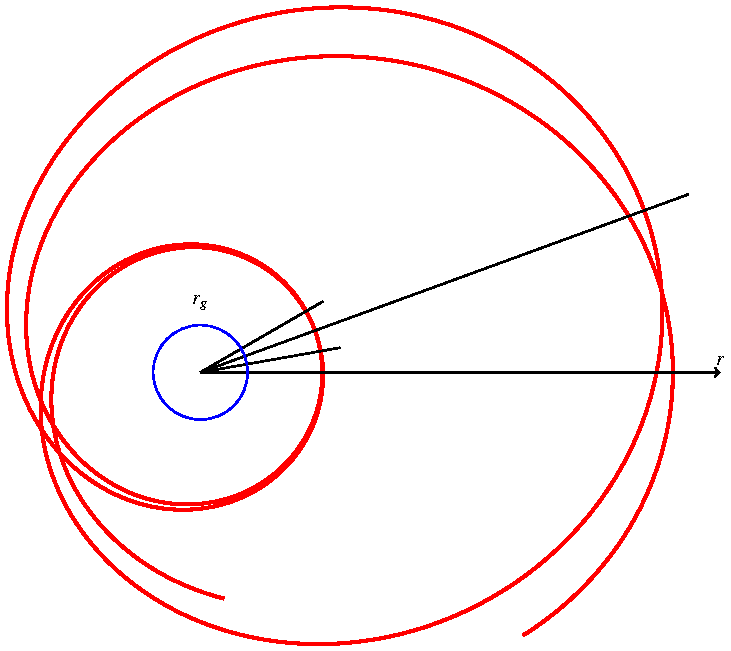
\includegraphics{chapters/tikz/orbit2.pdf}
\caption{Periheldrehung für eine Bahn, die sehr nahe an den Gravitationsradius
heranführt.
Anfangsbedingungen dieser Bahn sind
\eqref{skript:schwarzschild:anfangsbedingunge:extrem}.
\label{skript:schwarzschild:apside:extrem}}
\end{figure}
Bahnen, die sehr nahe an den Ereignishorizont heranführen, erfahren eine
noch viel deutlichere Drehung der Apsidenlinie.
In Abbildung~\ref{skript:schwarzschild:apside:extrem}
ist eine Bahn dargestellt, die sich auf weniger als $3r_g$ dem Zentralkörper
nähert.
Schon der Winkel $\varphi$ für das Perihel unterscheidet sich um um mehr
als $180^\circ$ vom Winkel $180^\circ$, der für eine Kepler-Bahn zu
erwarten wäre.
Die Anfangsbedingungen dieser Bahn sind
\begin{equation}
%    0.00000
%   10.00000
%    1.57080
%    0.00000
%    1.07220
%    0.00000
%    0.00000
%    0.01861
\begin{aligned}
t(s)        &=\phantom{0}0.00000                    &\dot t(s)         &= 1.07220\\
r(s)        &=          10.00000                    &\dot r(s)         &= 0.00000\\
\vartheta(s)&=\phantom{0}1.57080=\textstyle\frac\pi2&\dot \vartheta(s) &= 0.00000\\
\varphi(s)  &=\phantom{0}0.00000                    &\dot \varphi(s)   &= 0.01861
\end{aligned}
\label{skript:schwarzschild:anfangsbedingunge:extrem}
\end{equation}
